%===============================================================================
% $Id: ifacconf.tex 19 2011-10-27 09:32:13Z jpuente $  
% Template for IFAC meeting papers
% Copyright (c) 2007-2008 International Federation of Automatic Control
%===============================================================================
\documentclass{ifacconf}

\usepackage{graphicx}      % include this line if your document contains figures
%\usepackage{natbib}        % required for bibliography
\usepackage{nomencl}
\usepackage{amsmath}
\usepackage{natbib}
%\usepackage{citep}
\makenomenclature
%===============================================================================
\begin{document}
\begin{frontmatter}

\title{Application of Adaptive Network Approach for Power Grid Operations: Synchronization, Clustering And\\ Self-organized Criticality} 
% Title, preferably not more than 10 words.

\thanks[footnoteinfo]{Madhavi Parimi is Research Scholar at Electrical Engineering Department (EED), VJTI, Mumbai.}

\author{Madhavi Parimi} 
%\author{Sushama Wagh} 
%\author[First]{Ragini Meshram}
%\author[First]{Faruk Kazi}
%\author[First]{Navdeep Singh}


\address{Electrical Engineering Department, 
   Veermata Jijabai Technological Institute, Mumbai, India (e-mail:madhaviparimi7@gmail.com)}

\begin{abstract}                % Abstract of not more than 250 words.
The dynamics of a non-linear system are governed by either change in its states or in the network topology. Though both the approaches have been independently used in literature for different applications, the dynamics when both are considered together forms the basis for explaining various phenomena across diverse fields. It has been observed that the complexity of a non-linear system is due to the interplay between the states and the underlying topology, which leads to an adaptive network. This has motivated the authors to realize the existence of similar mechanism in the context of a power grid. The major contribution of this paper is to propose an adaptive framework to comprehend several phenomena in a power grid, viz. self-organized criticality, synchronization and cluster formation.  The control efforts to restore the power grid to a stable operating point can be viewed as an outcome of adaptation of the states as well as the topology. Also the presence of adaptive coupling drives the system into a stable state of clusters with equal or unequal number of oscillators, which is proposed to be further taken up to explain the occurence of inter-area oscillations.
\end{abstract}

\begin{keyword}
%Cyber Physical System, Induction Motor, Vector Control, Luenberger Observer, OPAL-RT
Adaptive Network, Complex Network, Kuramoto model, Non-linear dynamics, Power Grid, Synchronization
\end{keyword}

\end{frontmatter}
%===============================================================================

\section{Introduction}
%This document is a template for \LaTeXe. If you are reading a paper or
%PDF version of this document, please download the electronic file
%\texttt{ifacconf.tex}. You will also need the class file
%\texttt{ifacconf.cls}. Both files are available on the IFAC web site.
%
%Please stick to the format defined by the \texttt{ifacconf} class, and
%do not change the margins or the general layout of the paper. It
%is especially important that you do not put any running header/footer
%or page number in the submitted paper.\footnote{
%This is the default for the provided class file.}
%Use \emph{italics} for emphasis; do not underline.
%
%Page limits may vary from conference to conference. Please observe the 
%page limits of the event for which your paper is intended.
The study of complex systems involves interactions between its sub-systems resulting in the emergence of collective behaviour, attempts of perceiving which have been the driving force for developments in science and engineering. Examples of complex systems in real-life are the world wide web, social networks, biological protein networks, transportation networks, power grid etc. Numerous ways of modeling these systems help in analyzing their structure and behaviour. They exhibit unique spatio-temporal characteristics, which have rendered them as highly attractive targets of exploration. However, the research carried out to comprehend the structure and the dynamics of complex systems have been carried out in isolation. Combining these two under one modeling paradigm brings in a new persepctive of understanding several existing phenomenon. To this end, modeling of complex systems as an \textquotedblleft adaptive network\textquotedblright  will prove to be very insightful.\\
A network is treated as a structure comprising of nodes and links, which are interacting based on certain rules. If the network remains static while the states of the dynamical system are evolving, then such networks are known as dynamics on networks $(DoNN)$ as shown in Fig \ref {fig:2}. An important application that is studied within this framework include synchronization of the individual dynamical systems \citep{Strot}.
\begin{figure}[h!]
\begin{center}
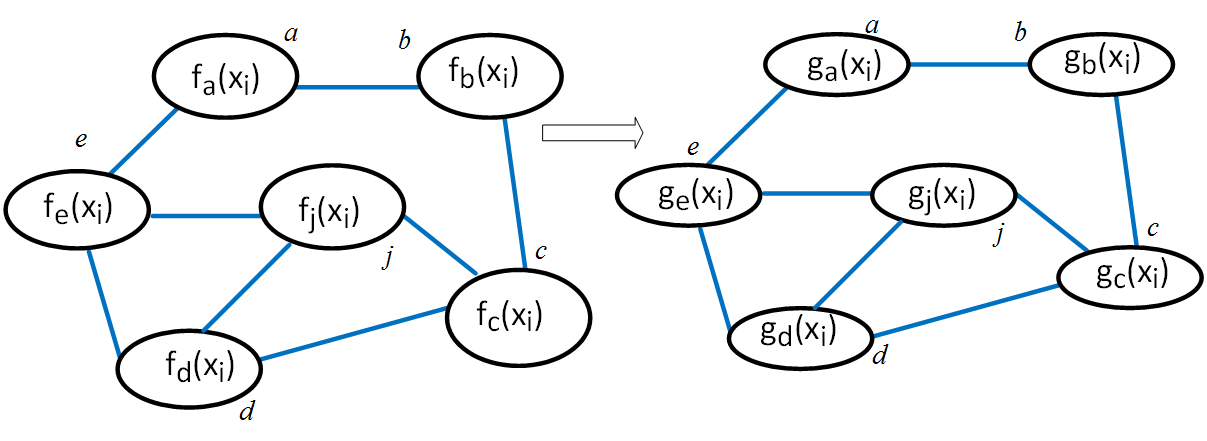
\includegraphics[width=7cm,height=3cm]{fig2.png}
\caption{Dynamics on Network (DoNN)}
\label{fig:2}
\end{center}
\end{figure}
The other line of research is concerned with the dynamics of networks $ (DoFN) $ as shown in Fig \ref {fig:1}. Here, the topology of the network itself is treated as a dynamical system, which keeps evolving with time according to certain rules or laws. Such an evolution would lead to peculiar network topologies with special properties. Notable examples include the formation of small world and scale-free networks.\\
\begin{figure}[h!]
\begin{center}
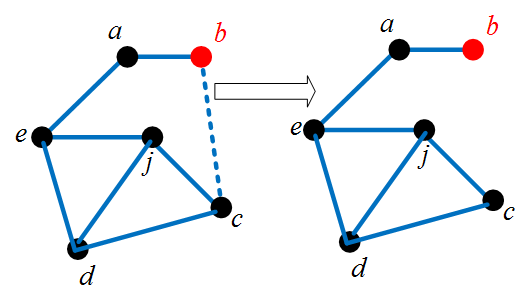
\includegraphics[width=6cm,height=4cm]{fig1.png}
\caption{Dynamics of Network (DoFN)}
\label{fig:1}
\end{center}
\end{figure}
For the purpose of analysis, the $(DoFN)$ and $(DoNN)$ are treated exclusive of each other in literature, as they evolve at different time scales. However, considering both the dynamics together can drive the system to a steady state that differs from the one obtained when the two processes are considered separately \citep{Cap}. Combining the two results in equilibria which are an outcome of the dynamical interplay between the state and the topology of the network. The main motive of this work is to view certain mechanisms in the power grid as a consequence of interactions between the dynamics of the network and the topology. Certain traits like self-organized criticality, synchronization and clustering can be explained better by considering the coevolving dynamics between the topology and the behaviour of the system. An adaptive network modeling forms a strong link in undertsanding these mechanisms. \\
The paper is organized as follows: Section II discusses the general framework of an adaptive network and the dynamical equations governing them. Section III  discusses the classical swing equation and the flux-decay model in the context of an adaptive synchronization using the Kuramoto model. The self-organized criticality (SOC) and application of adaptive network theory to it is discussed in Section IV. Section V depicts how adaptive coupling introduced by variation in coupling strength will result occurence of clustesr in a power network.
Section VI summarizes the discussion and proposes the conclusive remarks and future scope.\\
\section{Adaptive network theory}
This section focuses on how researchers have modeled power grid as DoNN and DoFN.   
Many systems in nature can be described by models of complex networks, which are structures consisting of nodes and edges. Initially, a complex network was modelled as regular shape such as an Euclidian lattice.
In the 1950s, Erdos and Renyi (ER) described a complex network as a random graph, though intuition tells us that many real life complex networks are neither completely random nor completely regular.
Later on, with increase in computational facilities and the size of the networks, two discoveries to model complex networks evolved: the small world  model and the scale free model. In order to describe the transition from a regular lattice to a random graph, Watts and Strogatz (WS) introduced the concept of small world networks. A common feature of the ER and the WS models is that the connectivity distribution of a network peaks at an average value and decays exponentially: hence they’re called exponential or homogeneous networks, because each node has about the same number of edge connections. Another model has evolved from the observation that many real large scale complex networks are scale free i.e. their connectivity distributions are in a power law form i.e. most nodes have very few link connections and yet a few nodes have many connections: inhomogeneous in nature. \\
\indent In the past few years, a number of large blackouts have led to an increasing interest in the study of bulk power grid. The topology of a power grid is critical in assessing its vulnerability to cascading failures.
As a type of a complex network, many power grids show the characteristic of a scale free network.
In a power grid, there are always a few central buses with high economic or geographic significance; in the planning, these buses are supposed to hold more links than the other buses.
The characteristics of evolution of power grid contributes to few nodes with high degree.
This scale free characteristic of a power grid makes it robust to random attack but fragile to intentional attack. The   methods of modeling discussed so far fall under the category of DoFN. Topological metrics such as average path length, clustering co-efficient, degree distribution etc are crucial in deciding the emergence of a blackout.\\
The power grid is modeled as DoNN when trying to address issues of transient stability assessment. The dynamics of the rotor of the generator described by the swing equation, gives a balance between the mechanical output of the rotor and the coupling of this output to the other nodes of the grid. The rotational properties of generators help in visualizing them as oscillators whose dynamics are governed by the Kuramoto model. The analogy between the swing equation and the oscillator dynamical equation is derived from the fact that both are a consequence of Newton's second law and are related to the active power flow. Solutions to Kuramoto model results in estimating synchronization of oscillators whereas solutions to swing equations involve determination of rotor angle stability. The motivation to symbolize machines as oscillators is to view phase locking of oscillators as synchronization of the rotor angles. The equivalence between the two dynamical equations has been explored by \citep{Dor}.\\
This paper wishes to propose that both the modeling approaches: of an evolving network and the transient stability assessment fall under the much broader framework of an adaptative network. 
An adaptive network is treated as a dynamical system with three functions $f$, $h$ and $g$, depicting the dynamics of the node, the relation showing the interaction between nodes and the adaptation rule respectively \citep{De}.\\
\begin{align}
\dot x &=f(x,t,u,A)\\
\dot a &=g(t,a,v,x)
\end{align}
where $A$ is the time varying adajecency matrix describing the network topology and $u \epsilon \Re^m$ is the input on the network nodes, $v \epsilon \Re^l$ is the input on interconnetion matrix described by the vector $a$ of nonzero elements of $A$ ($i.e.$ the set of active edges of the network). According to this framework, denoting $\sigma_{ij} $ as the adaptive gain associated with non-zero elements of A, the adaptive synchronization problem can be written as:
\begin{align}
\dot x &=f(x_{i},t)+\sum_{j \epsilon \varepsilon_{i}} \sigma_{ij}(t) [h(x_{j})-h(x_{i})] \\ \nonumber
\dot \sigma_{ij} &=g(t,\sigma_{ij},x_{i},x_{j})
\end{align}
where $ \varepsilon_{i} $ is the set of links beginning with $i$.
The choice of the functions $f$, $g$ and $h$ would depend on the application of interest. \\
%The former is where the power network attains self - organized criticality which is the outcome of adaptive nature of the %network. The latter approach is more relevant to attainment of stability of the system following a disturbance. The %original model proposed by Kuramoto can be extended to show the adaptive nature of the power grid. The second %contribution of the paper is to use this new model to address the following: 
This work proposes to view power systems as adaptive networks, from three different perspectives:
\begin{enumerate}
\item Synchronization
\item Self-Organized Criticality
\item Clustering or island formation
\end{enumerate}
\section{Adaptive Approach to Synchronization}
The phenomenon of synchronization is ubiquitous in nature and a very widely explored area from the point of view of applications in sciences and engineering. As stated in \citep{Pikov}, synchronization is the alignment of rythms of oscillating objects due to their weak interactions. There are two notions in perceiving the mechanism of synchronization: the first in which the dynamics of the system evolve to a particular solution due to their interactions with either the internal parameters or with the environment. And the second in which a desired trajectory has to be arrived upon, for which certain states of the system have to be controlled. The former is where the systems aligns in an organized way and in the process could attain a critical transition point. The latter approach has been widely applicable to tracking problems wherein different control strategies are proposed to synchronize the system. Therefore, phase transition and an organized behaviour are indigenous to synchronization. \\
 The modeling of a physical system into an oscillator involves certain assumptions, of which, the notion that they are identical is practically unrealistic.  A group of such non-identical oscillators will experience interacting forces which are weak. \citep{Weak} exemplify that the key to synchronization are the weak interactions between the non- identical oscillating objects. The work of Winfree and Kuramoto have used models with weak interaction between oscillators to achieve phase synchronization. \\
To achieve this, the underlying dynamical system has to be converted to a phase equation model which depicts the dynamics between the inherent oscillations of each oscillator and the interactions from the other oscillators. 
The Kuramoto model of synchronization is a very successful model to understand the synchronization of an ensemble of oscillators, wherein the coupling coefficient is assumed to be constant. However, variation in the coupling strength leads to an adaptive approach to synchronization as proposed in \citep{Kurths}. The Kuramoto model has been applied to address the transient stability problem of power systems, which is by large treated as a subclass of the synchronization problem. \\
The assessment of rotor angle stability is extremely crucial to measure the effect of large disturbances on the system. There have been two schema of bringing in synchronization of rotor angles, one is the series control (using FACTS devices like UPFC, TCSC) and the other is using excitation control at the generator nodes. The earlier method achieves global synchronization, whereas the latter ensures only enhancement in synchronization. Both the schemes are discussed in the following sections.\\
\vspace{-1em}
\subsection{The Classical Model : Kuramoto oscillators}
In a power network comprising of $n$ generator nodes, and $m$ load nodes, for transient stability assessment, rotor dynamics of generators need to be monitored, which can be represented by swing equations of generator $i$ as:
\begin{align} \label{eq:1}
M_{i}\ddot{\delta}_{i}=P_{mi}-E_{i}^{2}G_{ii}-D_{i}\dot{\delta_{i}}-P_{ei},\quad for\;i \in \lbrace1,\cdots,n \rbrace
\end{align}
where, internal voltage of generator $E_{i}>0$, mechanical power input $P_{mi}>0$, inertia $M_{i}>0$, damping constant $D_{i}>0$.
The electrical power output $P_{ei}$ is given as:
%\begin{equation} \label{eq:2}
\begin{align}
P_{ei} &= \sum_{j=1}^{n}\vert E_{i}\vert\vert E_{j}  \vert[Re(Y_{ij})cos(\delta_{i}-\delta_{j})+  \nonumber \\ 
& Im(Y_{ij})[sin(\delta_{i}-\delta_{j})] \nonumber\\
&=\sum_{j=1}^{n}\vert E_{i}\vert\vert E_{j} \vert \vert Y_{ij} \vert sin(\delta_{i}-\delta_{j})+\psi_{ij}] 
%\end{equation}
\end{align} 
%\end{small}
\begin{align}\label{eq:3}
where \; \vert Y_{ij} \vert=\sqrt {G_{ij}^2+B_{ij}^2} ,\;\;
\psi_{ij} =arctan(G_{ij}/B_{ij})
\end{align}
\indent Each oscillator oscillates independently at its natural frequency while the coupling tends to synchronize it to all others. When the coupling is weak, oscillators run incoherently whereas for coupling strength beyond a certain threshold, oscillators are synchronized with each other.  The governing equations of the coupled Kuramoto oscillator as shown in Fig \ref{fig:3} are:
\begin{figure}[h!]
\begin{center}
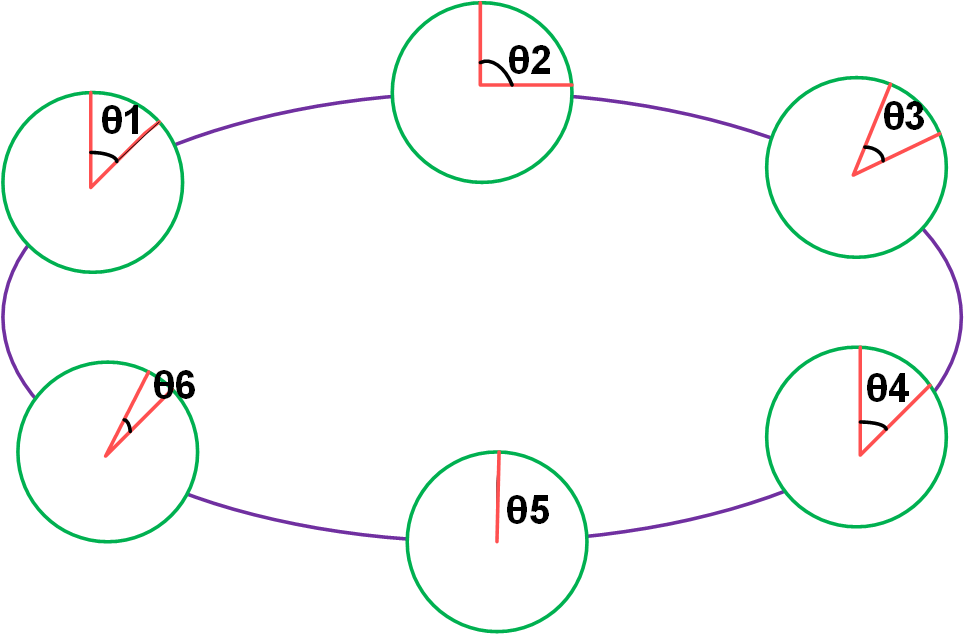
\includegraphics[width=6cm,height=4cm]{kura.png}
\caption{Coupled Oscillators}
\label{fig:3}
\end{center}
\end{figure}
\begin{align} \label{eq:5}
\dot \theta_{i}=\omega_{i}-\sum_{j=1}^{N} K_{ij} sin (\theta_{i}-\theta_{j}),  for\;i \in \lbrace1,\cdots,N \rbrace 
\end{align}
%\begin{figure}[H] 
%\centering
%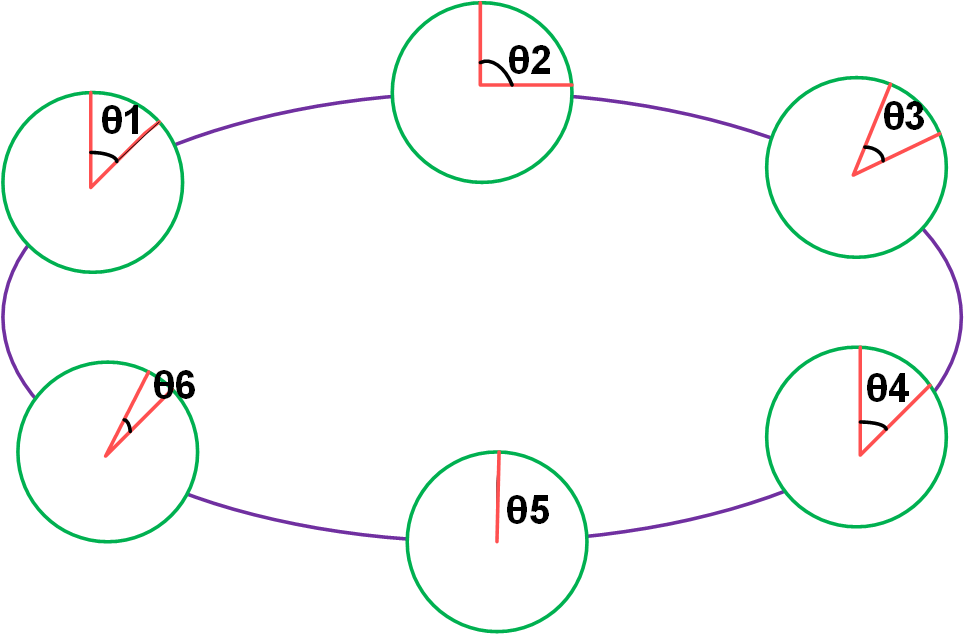
\includegraphics[scale=0.2]{kura.png}
%\caption{Kuramoto model of N coupled oscillators}
%\label{fig:1}
%\vspace{-.3em} 
%\end{figure}
%\vspace{-1.0em}
$K_{ij}$ is a matrix comprising of the coupling weights. In order to apply the Kuramoto model in power system parlance, the relationship between the power network model and a first-order model of coupled oscillators is exploited. 
The singular perturbation analysis is applied to show the congruity between (\ref{eq:1}) and (\ref{eq:5}), assuming that the generators are overdamped possibly due to local excitation controllers.
Using the relation (\ref{eq:6}) and (\ref{eq:7}) to represent the effective power input to generator $i$ and the coupling weights representative of power transferred between generator $i$ and $j$ respectively, (\ref{eq:1}) would get modified to (\ref{eq:8})
%\vspace{-1.0em}
%\begin{small}
\begin{equation} \label{eq:6}
w_{i} \equiv (P_{mi}-E_{i}^{2}(G_{ii}))
\end{equation}
\begin{equation} \label{eq:7}
P_{ij}=\vert E_{i}\vert\vert E_{j}\vert \vert Y_{ij} \vert \quad with \quad P_{ii}=0
\end{equation}
\begin{equation} \label{eq:8}
M_{i}\ddot{\delta_{i}}=-D_{i}\dot{\delta_{i}}+\omega_{i}-\sum_{j=1}^{n}P_{ij}sin(\delta_{i}-\delta_{j}+\psi_{ij})
\end{equation}
For small inertia over damping ratio ($\frac{M_{i}}{D{i}}$) of generators, singular perturbation can be applied to seperate slow and fast dynamics of the system, then (\ref{eq:8}) reduces to,
%\begin{small}
\begin{equation} \label{eq:9}
D_{i}\dot{\delta_{i}}=\omega_{i}-\sum_{j=1}^{n}P_{ij}sin(\delta_{i}-\delta_{j}+\psi_{ij})
\end{equation}
%\end{small}
which captures the power system dynamics sufficiently well during first swing. A corelation between (\ref{eq:5}) and (\ref{eq:9}) reveals that with $\psi_{ij}=0$, they both are alike, where $P_{ij} $ plays the same role as that of the coupling function $K_{ij}$. 
An intuitive representation of synchronization is brought about by the Kuramoto mean field model (KMFM), by taking $K_{ij}=K/N>0$, resulting in:
\begin{equation}\label{eq:10}
\dot \theta_{i}=\omega_{i}-\frac{K}{N} \sum_{j=1}^{N} sin (\theta_{i}-\theta_{j}),  for\;i \in \lbrace1,\cdots,N \rbrace 
\end{equation}
Equation (\ref{eq:10}) can be written in a more convenient form using the order parameter (OP) $r$, the centroid of the oscillators, which is a
natural measure of synchronization and defined as:%shown in Fig1 \citep{Str}.
\begin{equation}\label{eq:11}
  r(e^{j\phi t})=\frac{1}{N}\sum_{k=1}^{N} e^{j\theta_{k}(t)} 
\end{equation}
where $r$ measures phase coherence of the oscillators and $\phi$ measures the average phase. Kuramoto model (\ref{eq:10}) represented in terms of OP as:
\begin{equation}\label{eq:12}
 \dot \theta_{i}=\omega_{i}-K r sin (\phi-\theta_{i}), for\;i \in \lbrace1,\cdots,N \rbrace 
\end{equation}
As $ K \rightarrow 0 $, oscillators oscillate with their own natural frequencies, resulting in OP $ r \rightarrow 0 $ as $ t \rightarrow \inf $, implying incoherent oscillators. When $K \rightarrow1 $, the oscillators are synchronized to their mean phase and $r \rightarrow1$. For OP between $ 0 < r < 1 $, a few of the oscillators are phase locked and remaining are spread around the circle. \\
%We need to look for frequency synchronization and phase cohesiveness.\\ 
%This work wishes to emphasize that the synchronization phenomenon can be viewed as an application of an adaptive %network. 
When a fault occurs in the system, (\ref{eq:10}) is analyzed to assess the violation of rotor angles and calculate suitable control. This is achieved by inserting FACTS devices, which leads to modifying the $ Y_{ij} $ in (\ref{eq:7}). Eventually, this would result in change in line flows, thereby, ensuring synchronization of rotor angles. This is an adaptive approach to synchronization, where the change in topology changes the dynamics of the states. \\
\vspace{-1em}
\subsection{One axis Generator model with exciters }
This model includes one circuit for the field winding of the rotor, i.e., this model considers the effects of field flux decay \citep{Chiang}. As a result, the voltage behind the direct transient reactance is no longer a constant.
The adaptive network paradigm can also be extended to the flux decay model as in \citep{Chen}.
The third equation governing the dynamics of the exciter can be considered, in addition to (\ref {eq:12}):
\begin{equation}\label{eq:14}
\dot E_{i}=-a_{i}E_{i}+b_{i} \sum _{j=1,j \neq i} E_{j} cos(\delta_{i}-\delta_{j} )+E_{fij}+u_{i}
\end{equation}
where \\
\begin{equation}
b_{i}=\frac{1}{T_{di}} (x_{di}-x_{di}^{'})Y_{ij} ; \\ \nonumber
a_{i}=\frac{1}{T_{di}}[1-B_{ii}(x_{di}-x_{di}^{'})]  \nonumber
\end{equation}
The reader is suggested to refer \citep{Ort} for notations and symbols used in (\ref{eq:14}).\\
It can be observed that as $E_{i}$ changes, eventually, with respect to \ref{eq:7}, $P_{ij} $ can be varied. Therefore, 
a feedback mechanism from $ E_{i}$ is changing the coupling weights of the network, thereby altering the dynamics of the oscillator, aiding in the enhancement of synchronization. Hence, the process of achieving rotor angle stability is inherently an adaptive phenomenon, irrespective of the control method used.  
\section{Self-Organized Criticality} 
The (SOC) is a consequence of the adaptive nature of a complex network, wherein, it sets in a state of equilibrium which is marginally stable. As the system evolves from some intial condition, its interactions with the environment or its internal parameters results in a feedback mechanism driving the system to its critical value. 
Such a state is indicative of appearance of phase transitions, which could lead to the emergence of fractals. At a phenomenological level, SOC aims at explaining the tendency of open dissipative system to rearrange themselves in such a way to develop long-range temporal and spatial correlations \citep{Mei}. Even the slightest perturbation at the critical point would lead the system into an avalanche. Therefore, modeling of systems in the adaptive framework provide a better platform to perceive the spontaneous manifestation of the topological properties characterized by complex networks.\\
A power network is a continuously evolving network, the equilibrium of which keeps changing, based on the change in demand, generation or in the network topology. Either of these changes would eventually result in dynamics which affect both the connecting nodes as well as the dynamics of the network. As the load changes, the extra demand has to be met by the generator by changing the power angle at the machine. In this process, there could be a possibility that some of the lines may trip due to overload, thereby resulting in change in line flows, eventually leading to variation in the phase angles of the connecting buses. This mechanism of change in load is possible until the steady state power limit is reached, beyond which the system cannot take any further load and it collapses. \\
It has to be noted that the evolution mechanism of a power grid occurs at different time scales. Depending on the control motive, either the power system engineer is interested in solving the faster evolving power flow equations or the slow evolving rotor angles based on the swing equations. However, it would be of interest to consider the interaction between the two dynamics, as shown in Fig \ref{fig:4}.
\begin{figure}[h]
\centering
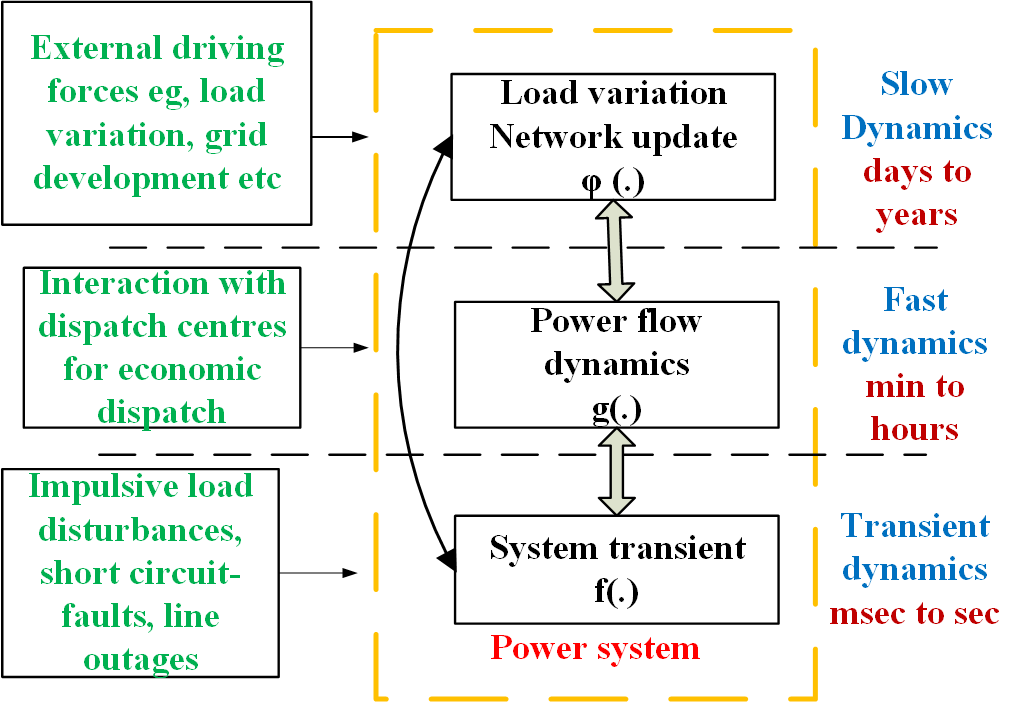
\includegraphics[scale=0.45]{power_evolution.png}
\caption{Evolution of power system }
\label{fig:4}
\end{figure}
The slow dynamics, which are long-term, are characterized by the existence of multiple equilibrium points and the system transits from one operating point to the other. The system at each juncture, tries to maintain a balance between the external ebergy supplied, the output delivered and the system losses. Therefore, its always in a transient state. However, the fast dynamics are governed by the constraints which are intrinsic to the system and can lead to catastrophic behaviour owing to presence of uncertainty.  Therefore, the slow and the fast dynamics cumulatively drive the system into a state of SOC. \\
The adaptive framework to model SOC in a power grid can be explained by the following Differential-Difference-Algebraic equations \citep{Mei}:\\
\begin{subequations}
%\label{eq:15}
\begin{align}
   \dot x &=f(x,y,s,u,w)  \\
  0 &=g(x,y,s,u,w)  \\
  s(t_{k+1}) &=\phi(x,y,s_{k}, u,w)\\
\end{align}
\end{subequations}
It is to be noted that {16a} indicate the transient dynamics of generators and loads, {16b} denote the  fast dynamics which are a set of algebraic equations governed by the real and reactive power flow constraints; and the set of
difference equations {16c} describe slow dynamics including
the load increase and power grid constructions. 
%Here $x, y, s, u ,w $ are the state, output, discrete parameters, control and disturbance respectively .
 The state $x$ comprises 
of the rotor angles and frequencies of the generators, the output $y$ includes
the bus voltages and the line flows through the transmission lines; the discrete
parameters $s$ are determined by the slowly changing dynamics of the system; the control $u$ consists of
the adjustments of generation outputs, relay actions, switches, and other preventive
and emergency control actions; the disturbances $w$ include short-circuit faults, incorrect
operation of dispatchers and misoperation of relays \citep{Mei}. \\
The combined set of (16) indicate how the power grid model evolves continuously, suggesting an adaptive mechanism involved in the emergence of an organized and a critical behaviour. 
\section{Cluster Formation}
The third application of adaptive network theory is with respect to the role played by adaptive coupling in the formation of clusters in a network of coupled oscillators. As proved in \citep{Kurths}, the introduction of adaptive coupling can induce the occurrence of multi-stable states (MSS) in a system of coupled oscillators. MSS implies: existence of two cluster state and a desynchronized or a splay state. It has also found that the weight of the coupling strength and the plasticity of the coupling play a crucial role in controlling the occurrence of MSS. From power system point of view, the existence of the two-cluster state is more relevant to corelate the formation of islands or clusters after a cascade failure happens. The analysis in this section helps in deducing that introducing adaptive coupling to the basic Kuramoto model results in a faster attainment of the two-cluster state.  \\
The standard Kuramoto model of phase oscillators:
\begin{equation} %\label{eq:10}
\dot \theta_{i}=\omega_{i}-\frac{K}{N} \sum_{j=1}^{N} f(\theta_{i}-\theta_{j}),  for\;i \in \lbrace1,\cdots,N \rbrace 
\end{equation}
$R_{1}$ is the coherence parameter which determines the coupling strength of the whole system.
\begin{equation}\label{eq:17}
  R_{1}=\frac{1}{N}\sum_{k=1}^{N} e^{j\theta_{k}(t)} 
\end{equation}
In case of adaptive coupling, $K=\sigma K_{i}$, where $\sigma$ is the strength of coupling and $ K_{i} $ are the coupling weights of oscillators. The coupling weights $K_{i}$ are considered to be dynamic, governed by the following dynamical equation:
\begin{align}\label{eq:18}
\dot K_{i}= \frac{\eta}{N} \sum_{j=1}^{N} g(\theta_{i}-\theta_{j})
\end{align}
where $g$ is a $2\pi$ periodic function called the plasticity function which determines how the coupling weigths depend on the relative timing of oscillators and $\eta$ is called the plasticity parameter. The choice of the functions $f$ and $g$ are the simple $ sin$ and $cos$ functions which modifies the dynamical equations to:
\begin{align}
\dot \theta_{i}=\omega_{i}-\frac{K}{N} \sum_{j=1}^{N} sin(\theta_{i}-\theta_{j}),\\ \nonumber
\dot K_{i}= \frac{\eta}{N} \sum_{j=1}^{N} cos(\theta_{i}-\theta_{j})
\end{align}
\begin{figure}[h!]
\begin{center}
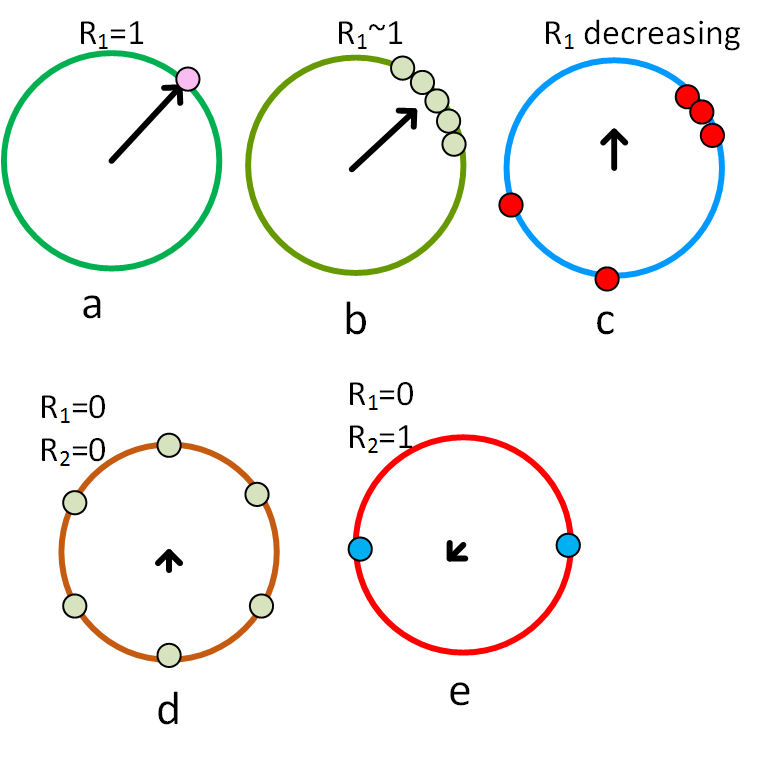
\includegraphics[width=8cm,height=6cm]{mss.png}
\caption{Synchronization regimes with variation in order parameters $R_{1}$ and $R_{2}$}
\label{fig:5}
\end{center}
\end{figure}
Before proceeding further, a few definitions are in order:
\begin{enumerate}
\item Synchronous state: A state in which the interaction between the oscillators is attractive and tends to lock them in-phase. Fig \ref{fig:5}a and Fig \ref{fig:5}b correspond to the phase synchronized and phase cohesive states. If all the oscillators are in the generating mode, then they are said to be phase cohesive. 
\item Partial synchronous state: A few oscillators are locked together while a few have moved out of the coupling as in Fig \ref{fig:5}c.
\item Splay state: A state wherein all the oscillators are spread uniformly along the circle as in Fig \ref{fig:5}d. 
\end{enumerate}
%\begin{figure}[H]
%\centering
%\includegraphics[scale=0.4]{states.png}
%\caption{Symmetric balancing of oscillators }
%\label{fig:4}
%\end{figure}
Here, $K=\frac{1}{N} \sum_i K_{i} $ is defined as the average coupling strength. Fig \ref{fig:5} shows how the variation in order parameters induces different modes of synchronization. Fig \ref{fig:5}a and \ref{fig:5}d showcase extreme conditions of order parameter, $R_{1}$, indicating phase synchronization and a splay state respectively. As one moves from Fig \ref{fig:5}a to \ref{fig:5}d, the coupling strength k decreases. Fig \ref{fig:5}c depicts a condition of partial synchronization, or a critical state, depicting the phase transition stage. As $K<K_{cr}$,  $R_{1}$ further decreases and would result in a splay state, wherein the oscillators are distributed all around the circle. However, the presence of plasticity parameter $\eta$ helps in formation of a two cluster state which is governed by the order parameter $ R_{2}$, given by:
\begin{align}
R_{2}= \frac{1}{N} \sum_{j=1}^{N} e^{2i \theta_{j}}
\end{align}
It has been proved in \citep{Kurths} that $R_{2}$ has to be equal to 1 so as to result in formation of the two cluster state. With  $R_{2}=1$, if  $R_{1}=0$, then each cluster has equal number of oscillators whereas if  $R_{1} \neq 0$, then each cluster has unequal number of oscillators. 
%Hence, the presence of $ \neta$ helps in faster attainment of the clusters, under the assumption that the initial %distribution of phases is random.???
It can be clearly seen from the figures that when the system splits up into islands, the rotor angles of the machines are perturebed from Fig \ref{fig:5}c and the presence of $R_{2}$ would aid in forming a two cluster state, rather than a splay state. Therefore, if the original system has to be restored, increase in $R_{1}$ results in a faster movement from Fig \ref{fig:5}e to \ref{fig:5}c, thereby resulting in a rapid attainment of synchronization. In short, $R_{1}$ controls the synchronization of the system, whereas the value of $R_{2}$ regulates oscillators to be in a group of two. This discussion emphasizes the role of adaptive coupling in the attainment of synchronization.
\section{Conclusions and future scope}
The adaptive approach of modeling complex systems helps in explaining various phenomenonin a power network. 
The adaptation between the slow and fast dynamics of the power grid makes it a resilient network. However, increase in load or generator outages drives the system into a self-organized state, perturbations to which are followed by blackouts. The paper has brought in a different view point to the traditional problem of transient stability assessment, stating that the control efforts to stabilize the system after a fault, are in a way, a consequence of an adaptive phenomenon. The mathematical framework that is central to this concept is the standard Kuramoto model. Another interesting application is that the presence of adaptive coupling would aid in cluster formation, which could result in saving the system from a complete collapse. *The future scope of this work is two fold: first is to extend these concepts and interpret their relevance in the context of a microgird . And secondly, it is envisaged that the paradigm of adaptive coupling would serve as a modeling framework to comprehend the phenomenon of inter-area oscillations
%\vspace{-1em}
\begin{ack}
The author is highly indebted to Dr S R Wagh and Dr. N M Singh, faculty members at EED, VJTI, for their valuable guidance and inputs throughout the work.The author would like to acknowledge the support of
Center of Excellence in Complex and Non-Linear Dynamical
Systems (CoE-CNDS), VJTI, Mumbai, India and TEQIP-II
(subcomponent 1.2.1).
\end{ack}

\bibliography{ifacconf_1Feb}             % bib file to produce the bibliography
 % \bibliographystyle{plain}                                      
                                        % Sections and subsections are supported  
 \printnomenclature
 \end{document}
